\documentclass[10pt]{article}
\usepackage[utf8]{inputenc}
\usepackage [english]{babel}
\usepackage [autostyle, english = american]{csquotes}
\MakeOuterQuote{"}
\usepackage{amsmath}
\usepackage{amsfonts}
\usepackage{amssymb}
\usepackage{graphicx}
\usepackage{subfig}
\usepackage[all]{nowidow}
\graphicspath{ {Images/} }
\usepackage{float}
\usepackage[belowskip=-20pt,aboveskip=0pt,font=normalsize]{caption}
\usepackage[backend=bibtex]{biblatex}
\bibliography{bib}

\DeclareFieldFormat{labelnumberwidth}{\mkbibbold{#1\adddot}}



\begin{document}

\title{\bf Employee Attrition: What Makes an Employee Quit?}
\author{
	Christopher Boomhower$^1$
	\and
	Stacey Fabricant$^2$
	\and
	Alex Frye$^1$
	\and
	David Mumford$^2$
	\and
	Michael Smith$^1$
	\and
	Lindsay Vitovsky\textsuperscript{1,2}
}
\date{}
\maketitle{}

\begin{center}
{$^1$ Southern Methodist University, Dallas, TX, US\\$^2$ Penn Mutual Life Insurance Co, Horsham PA}
\end{center}

%definition of quote with addition of [\textbf{Abstract --- ]
\renewenvironment{abstract}
               {\list{}{\rightmargin\leftmargin}%
                \item[\textbf{\hspace{10mm}Abstract.}]\relax}
               {\endlist}


\begin{abstract}\fontsize{9}\noindent Albeit to varying degrees, employee attrition is a costly challenge faced by many employers \cite{kantor}.  In this paper, we present a model for predicting employee attrition, as well as discuss the serious ethical implications of using such a model within organizations. To accomplish this, we examined publicly available data from the Office of Personnel Management, the Bureau of Labor Statistics, and IBM.  With these sources, we determined a set of statistically significant factors that correlate to an employee’s decision to quit, and determined to which types of occupations our model may be applied.  After applying Principal Component Analysis and classification methods K-Nearest Neighbors and Random Forest, it was Logistic Regression that allowed us to simplify the model and predict employee quits with the highest accuracy of our testing methods, achieving a greater than seventy-four percent success rate.  \end{abstract}

 
\section{Introduction}

\paragraph{How much does it really cost to lose an employee? Studies such as the Center’s for American Progress analysis (November, 2012) indicate a separated employee may cost between 16 to just over 213 percent of their annual salary, depending on the position \cite{boushey}. Precisely quantifying this may seem out of reach depending on the complexity of a particular role, but easily foreseeable areas of impact are: 1) determining if an employee’s vacancy should be replaced or duties handed off to others; 2) posting the job opportunity to various outlets; 3) interviewing, hiring, and training a replacement; 4) enduring lowered employee morale and possible lower productivity from 
 remaining employees; and 5) tolerating a lower skill set from an underdeveloped replacement \cite{kantor}.}

\subparagraph{Of course, many corporations are keenly aware of the downsides to losing employees.  As such, many exert great efforts to maintain retention levels, such as by providing substantial workplace benefits \cite{glassdoor}. Gaining an understanding of the reasons why employees separate certainly empowers Human Resource departments to improve retention through improved planning and intervention.  While such insights are available to organizations that store employee data, these understandings are not within reach without sufficient analysis.}

\subparagraph{The first step in gaining foresight into employee attrition is obtaining pertinent data. Companies are understandably reluctant to release the methods, proprietary or purchased, that use even anonymous data to help them in their management of human resources. Various articles allude to this challenge \cite{abellin}, \cite{richter}, \cite{walker}. However, we identified three valid sources of Human Resources data in the forms of Office of Personnel Management data, Bureau of Labor Statistics data, and the "IBM HR Analytics Employee Attrition" data set. All three forms were analyzed in unison to complement one another in insight and model validity.}

\subparagraph{Our process began with data sampling and traditional exploratory data analysis, but we quickly determined we would need to narrow our focus on these very large data sets which include many different types of variables.  We limited our scope to U.S. domestic, professional (white collar) jobs that have a General Schedule Equivalent of Level 7 or above (this is discussed in further detail within Section 2).  We also investigated the qualitative nature of these data to ensure that, at each step of data removal or dimensionality reduction, we were remaining on course to answer our ultimate question of interest, "What makes an employee quit?" Effects beyond the control of the employer or the employee (e.g. death) were carefully reviewed to properly apply and interpret our modeling techniques.}

\subparagraph{Our initial modeling techniques were classification methods that incorporated all variables, as we were still investigating which variables affected the decision to quit with statistical significance.  After eventually simplifying the data by keeping variables with high correlation to attrition responses and only focusing on responses within control of the employer (i.e. employers cannot control disabilities, deaths, etc), the models began to greatly improve.  Ultimately, it was logistic regression that provided us the most success, both intuitively and statistically.}

\section{Attrition as Seen in Civil Service Workers}

\paragraph{The U.S. Office of Personnel Management (OPM) serves as the central Human Resources department for all federal agencies, including the management of federal agency health insurance and retirement benefits. Their oversight of policy implementation, as well as being a general resource for all agency Human Resource departments, makes their employment data of particular interest for this paper. OPM releases, on a quarterly basis, updated separation data on its over two million federal civil service workers.  We used these anonymized data sets to create a full year of separation data, spanning October 2014 - September 2015.   These data \cite{opm}, include the following variables: 1) age group, captured categorically in 5-year increments (AGELVL and AGELVLT); 2) agency type and sub-type information (AGYTYP, AGYTYPT, AGY, AGYT, AGYSUB, and AGYSUBT); 3) gender (GENDER and GENDERT); 4) General Schedule Grade, or equivalent, dictating salary level (GSEGRD); 5) geographical location of the employee down to the state level (LOCTYP, LOCTYPT, LOC, LOCT); 6) length of service as a government employee captured in one-year increments until five years is achieved, then every five after that (LOSLVL and LOSLVLT); 7) occupation type  in regards to white or blue collar, occupation family, and in some cases, drilled down to the particular occupation itself (e.g. "chaplain") (OCCTYP, OCCTYPT, OCCFAM, OCCFAMT, OCC, OCCT); 8) occupation category among seven main categories (e.g. "Technical" and "Clerical") (PATCO and PATCOT); 9) pay plan and grade for both General Schedule Equivalent (GSE) and non-GSE occupations (PPTYP, PPTYPT, PPGROUP, PPGROUPT, PAYPLAN, PAYPLANT, and PPGRD); 10) salary range, captured categorically starting with less than \$20,000 and increasing in \$10,000 increments (SALLVL and SALLVLT); 11) reason for separation (SEP and SEPT); and 12) type of appointment and work schedules, denoting factors such as permanence, seasonality, and executive status (TOATYP, TOATYPT, TOA, TOAT, WSTYP, WSTYPT, WORKSCH, and WORKSCT).}


\subparagraph{There are certain points worth noting to understand our findings in the correct context.  The General Schedule (GS) Pay Scale is the centralized pay scale used by many civil service agencies. Even if a person is not paid under the GS, the OPM converts the level he or she is paid under to the GS for data collection purposes. The scale numbers 1-15, and there are ten "steps" within each of these levels.  Also, to remain competitive with industry salaries, the GS operates a locality adjustment scale that adds a particular percentage to a person’s salary, based on city of occupation alone.}

\subparagraph{Also, beginning on January 1, 1987,  new civil service employees were paid under the Federal Employees Retirement System (FERS). This mix of Social Security, a Basic Benefit Plan, and a Thrift Savings Plan helps make civil service positions stand out from many current private sector jobs in terms of retention. We account for this factor in our research, taking into consideration the confounding effect this has on length of service (LOS). At the time of this paper, the pension is based on salary and length of service.}


\section{OPM Data Consolidation, Sampling, \& New Attributes}

\paragraph{Our research focuses on the following employee types, only using observations that fit the following rubric: 1) domestic workers (no international positions), 2) employees aged 20 and greater, 3) employees with a job grade level greater than 7 (i.e. white collar only), and 4) only those who are considered full-time employees (i.e. no contracted, temporary, or part-time employees).}  
  
 
\subsection{Data Removal}

\paragraph{After reviewing the percentage representation of the various occupation types, as well as investigating the types of jobs that comprise each grouping, we kept only Professional and Administrative positions. Figure~\ref{fig:PATCOTOccCounts} depicts the overall record counts present within our data set by occupation category type. As observed, there are more employees of Administrative and Professional occupation types than any other category. Reviewing separation type ratios which comprise these total counts provides further insight and justification into why Professional and Administrative jobs are targeted within this paper.}

\subparagraph{}
\begin{figure}[H]
\centering
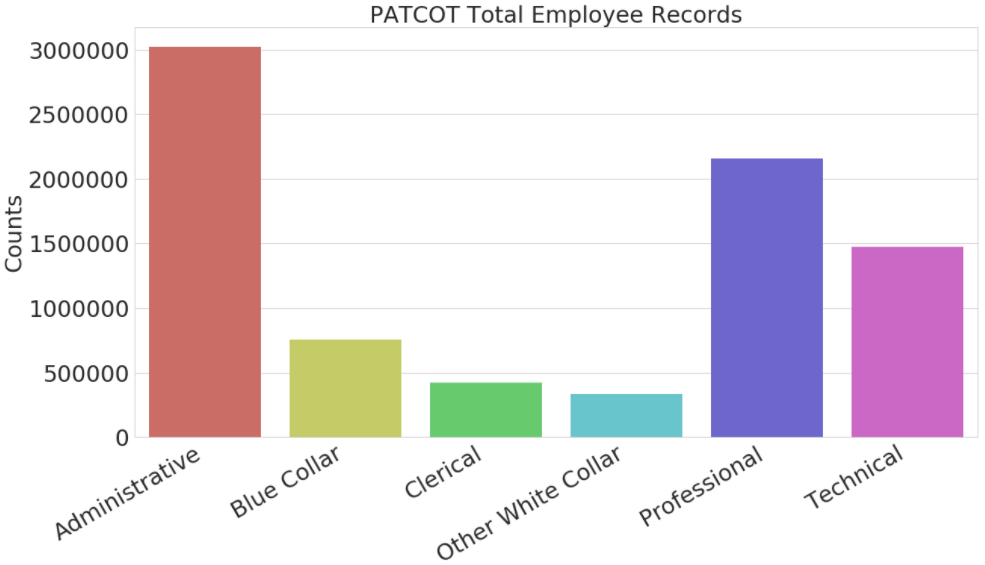
\includegraphics[width=\linewidth]{PATCOTOccCounts.png}
\caption{Occupation Category Type – Observation Counts}
\label{fig:PATCOTOccCounts}
\end{figure}

\subparagraph{The percentage plot of Figure~\ref{fig:PATCOTSepPercentages} indicates the distribution of separation types within each occupation category. Note for improved granularity, non-separated employee data has been removed from the visualization as there are far more employees remaining at work than there are leaving, which therefore skews plotted results. So, only true separations are represented visually.}

\subparagraph{}
\begin{figure}[H]
\centering
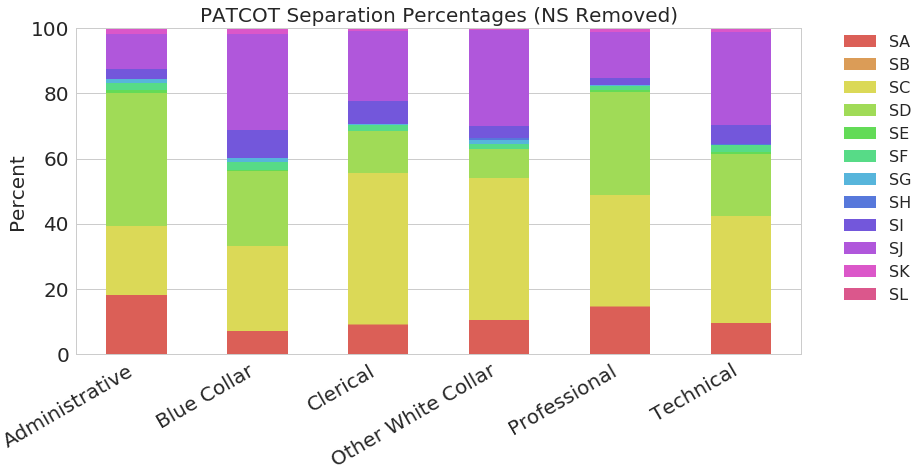
\includegraphics[width=\linewidth]{PATCOTSepPercentages.png}
\caption{Occupation Category Type – Separation Percentages with NS Removed}
\label{fig:PATCOTSepPercentages}
\end{figure}
 
\subparagraph{As Figure \ref{fig:PATCOTSepPercentages} illustrates, approximately the same number of Professional employees who retired (SD) in this time frame quit (SC) as well. Treating retirement as a proxy indicator for retention, this even distribution of quits vs. retirements suggests great retention rates among Professional employees and aligns with non-separation counts as well. Similar argument is to be made of Blue Collar jobs also, and the combination of individual transfers out (SA) and quits is approximately the same in size as retirements for Administrative types. However, the Professional category type was identified as a better candidate for primary model application due to its large total count, as discussed previously, in combination with its more widely diverse professional job types that more closely resemble private sector occupations. Nonetheless, due to its high employee count, strong retention numbers, and similar transfer and quit counts compared to retirements, the Administrative occupation category was selected as secondary target for modeling purposes as will be discussed further in Section 5. Therefore, data for all occupation category types, except Professional and Administrative, were removed from our data set.} 
 
 
\subsection{OPM Computed Attributes}

\paragraph{Seven new attributes were created through aggregation or calculation: 1) SEP Count by Date \& Occupation – Total number of separations (of any type) for a given Date and Occupation; 2) SEP Count by Date \& Location – Total number of separations (of any type) for a given Date and Location; 3) Industry Average Salary – Average salary among non-separated employees, grouped by quarter, occupation, pay grade, and work schedule; 4) Lower Limit Age – Youngest age within each age level category; 5) Years to Retirement – Based on FERS retirement eligibility baseline of 57 years of age \cite{bls}; 6) Length of Service Square Root Transformation – Square root transformation to account for service length's skewed distribution; and 7) Salary Over/Under Industry Average – Difference between computed average salary of non-separated employees and actual salary for each observation. Another 1,293 observations were removed after calculating industry average salary, as they had no matching non-separation observations (matched on quarter, occupation type, pay plan/grade, and work schedule), which were utilized to ensure realistic salary averages.}
 
\subsection{Bureau of Labor Statistics Derived Attributes}

\paragraph{In addition to the OPM data, we merged 10 attributes from the Bureau of Labor Statistics (BLS). Data were sourced from Federal Government industry codes across all regions. Although assumed to be highly correlated, we sourced both Level (Total number) and Rate (Percentage of Level to total employment and/or job openings) for the following statistics: 1) Job Openings, 2) Layoffs, 3) Quits, 4) Total Separations, and 5) Other Separations. While Rate paints an aggregated, holistic picture for job market trends, Level provides a raw count for total separations alone. Both these statistics were captured by a monthly aggregate and merged to the OPM data by their respective months.}
 
\subsection{Sample Design}

\paragraph{Data were divided into groups based on separation type, allowing a maximum of 7,500 observations per type to persist forward during analysis. In so doing, the following retirement separation types were combined to create our Non-Separation (NS) group: 1) NS, Non-Separation; 2) SA, Transfer Out - Individual Transfer; 3) SB, Transfer Out - Mass Transfer; 4) SD, Retirement - Voluntary; 5) SE, Retirement - Early Out; 6) SF, Retirement - Disability; and 7) SG, Retirement - Other. Our Quit (SC) group is stand-alone in our analysis to serve as our main focus and goal for prediction. All other separation types were removed for analysis as they were either irrelevant to our goals or were due to uncontrollable events, such as death.}
 
\subparagraph{Within each separation group (including non-separation), proportional allocation was performed on a combination of date and age level strata to ensure a sample demographic which, as closely as possible, represents that of the original strata-level populations. After sampling, we were left with 14,920 observations in our primary data set for model generation. The secondary data set of Administrative occupations also contained these unbalanced strata, and thus the same sample design was implemented to reduce the data set to 14,918 observations.}
 
\section{Preliminary Analysis}

\paragraph{Reviewing the final Professional occupation category data provided lead indicators that assisted us in creating our primary attrition model. The findings described below guided our approach to model generation as they suggest some attributes do truly correlate more strongly with attrition than others. These findings also serve as primer to our feature importance analysis as will be described in Section 5.}
 
\subparagraph{}
\begin{figure}[H]
\centering
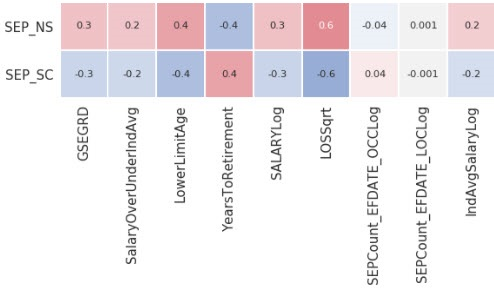
\includegraphics[width=\linewidth]{SEP_CorrMatrix.jpg}
\caption{Numeric Attribute and Separation Type Correlation Matrix}
\label{fig:SEP_CorrMatrix}
\end{figure}

\subparagraph{As indicated in Figure~\ref{fig:SEP_CorrMatrix}, there are several intuitive observations to be made of the correlation values shared by separation type and the remaining quantitative attributes present in the data set. Note numerical values shown are Pearson’s correlation coefficient values. The most noteworthy mention identified in the correlation matrix is that Separation (SEP\_NS) is positively correlated with length of service (r = 0.6). Though expected, this is still worth noting as it supports the prospect of retiring with benefits, as opposed to quitting, can help entice an employee to stay. Of course, the pension calculation is heavily based on number of years of service, so it is unsurprising that length of service is the highest positively correlated factor for non-separated employees.}
 
\subparagraph{The correlation values for separation from quitting (SEP\_SC) in Figure~\ref{fig:SEP_CorrMatrix} is what interests us most.  As general schedule grade (GSEGRD) decreases, the likelihood of separation by quitting increases (r = -0.3). This makes logical sense, as schedule grades are directly tied to income.  However, this correlation also exactly matches the correlation for the employee salary, so there is not enough direction to say that the status of the schedule grade matters moreso than the actual salary. Though not indicated in Figure~\ref{fig:SEP_CorrMatrix}, salary and schedule level do, in fact, strongly correlate with one another (r = 0.9). As such, the two are most likely one-and-the-same in an employee's mind, and only one of the two will be used for modeling purposes.}
 
\subparagraph{Finally, the correlation of quits to years until retirement eligibility is positively correlated (r = 0.4); the further someone is from being able to retire, the more likely they are to quit. But when considering the correlations observed for schedule grade and salary, a key takeaway is that the job positions for which it is more difficult to replace and train should be assigned higher schedule grades and lower income differentials from industry. This conclusion aside, these insights solidified our data as being predictive of attrition.}

\section{Modeling and Evaluation}

\paragraph{Methodologies Logistic Regression, Random Forest, and K-Nearest Neighbor (KNN) were implemented to predict separation types amongst our sampled professional occupations. Four disparate feature input selections were utilized in attempts to reduce dimensionality in our initial input of 99 attributes. Ultimately, Logistic Regression produced most effective trained results and the generated models were applied to a different demographic of Administrative occupations.}
 
\subsection{Feature Input Selections}

\paragraph{Four feature input selections were made during the modeling process in search of the best features for each model type. Selections made were: 1) Full 99 Raw Scaled Value Features; 2) Principal Component Analysis (PCA) Eigenvector Matrix; 3) Top 15 Raw, Scaled Features within each PCA loading; and 4) Manual Logistic Regression Feature Selection.  These four selections are further explained below:}

\subparagraph{\textit{Full 99 Raw Scaled Value Features}: All 99 values after Min-Max Scaling were included.}

\subparagraph{\textit{Principal Component Analysis Eigenvector Matrix}: PCA was performed on our professional occupation samples in attempts to reduce our 99 input attributes. As can be seen in Figure~\ref{fig:PCA_Scree_CumVar}, the percentage of explained variance leveled out around 22 components, at which point cumulative explained variance approached 80\%. These 22 principal components were utilized as a data set of component vectors.}

\subparagraph{}
\begin{figure}[H]
\centering
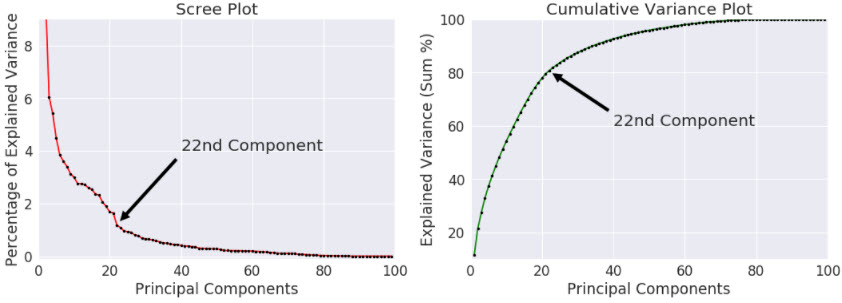
\includegraphics[width=\linewidth]{PCA_Scree_CumVar.jpg}
\caption{Explained and Cumulative Variance Plots}
\label{fig:PCA_Scree_CumVar}
\end{figure}

\subparagraph{\textit{Top 15 Raw Scaled Features within Each PCA Loading}: Utilizing the PCA analysis performed above, the top 15 features within each of the 22 components were identified through absolute loading magnitudes. This reduced our inputs to 46 features, allowing only the most important features to proceed into our model as raw, scaled values based on PCA loadings.}

\subparagraph{\textit{Manual Logistic Regression Feature Selection}: Important independent variables were identified by first assessing multicollinearity and covariance among the 99 raw features, and then iteratively generating logistic regression models - removing one feature at a time with each iteration. Removal criteria were based on Variance Inflation Factor (VIF) values (Threshold for removal was VIF of 10), Null Deviance, Log Likelihood, Akaike Information Criterion (AIC), Bayesian Information Criterion (BIC), and p-values ($\alpha = 0.05$). Only statistically significant features remained for model input after completing this process (32 variables in total).}
 

\subsection{Classification Model Training and Comparison}

\paragraph{To train our model, we utilized Stratified K-Fold Cross Validation for our classification analysis, with five folds. From our original sample size of 14,922, each fold, or iteration, was split approximately 20\% as test observations, utilizing the rest as training observations all while keeping the ratio of classes equal among separation types. These folds allowed us to validate that we are not overfitting our model and increase our understanding of whether our model may hold up for external data sets.}

\subparagraph{Among the three model types and four separate input features tested, Logistic Regression with manual feature selection was identified as having the greatest overall accuracy. As depicted in Table~\ref{fig:AccTable}, the winning model produced an average accuracy of 74.595\%, closely followed by Random Forest using the same feature inputs at 74.119\%.} 

\subparagraph{}
\begin{table}[H]
\centering
\caption{Raw Accuracy Data for Top 4 Model Results}
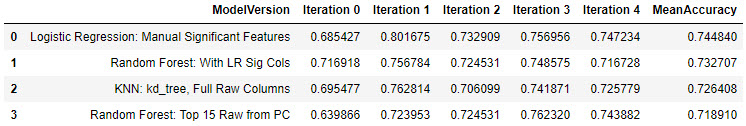
\includegraphics[width=\linewidth]{AccTable.jpg}
\label{fig:AccTable}
\end{table}

\begin{figure}[H]
\centering
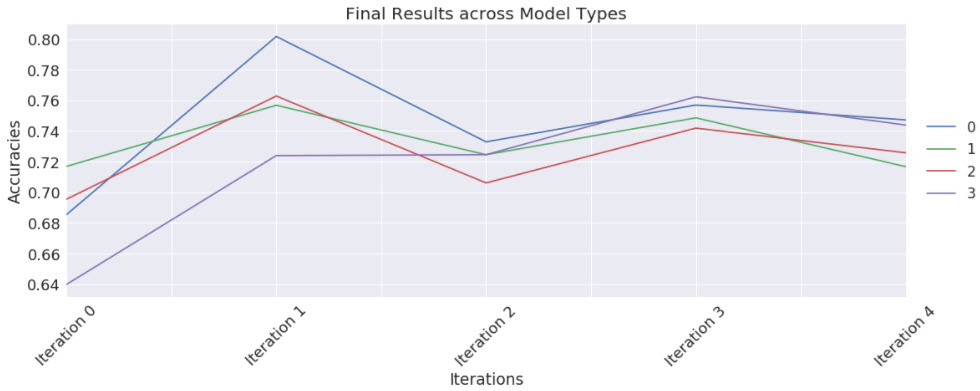
\includegraphics[width=\linewidth]{AccPlot.jpg}
\caption{Accuracies Across Test Folds for Top 4 Model Results}
\label{fig:AccPlot}
\end{figure}

\subparagraph{Furthermore, we see visually in Figure~\ref{fig:AccPlot} that the variation in accuracy for each model across the five fold tests further supports the Logistic Regression results as a strong selection. Legend indexes, matching those found in Table~\ref{fig:AccTable}, show Logistic regression as the winner among 2/5 iterations, and a close second only trailing behind 0.4020\% and 0.4692\% in iteration 2 and 3, respectively. Interestingly, the disparate feature inputs to the Random Forest model created vastly different results, with the top 15 PC features producing very inconsistent results across folds. With large differences in results between the first two folds, we push further into True Positive / False Positive rates to ensure we do not have too large of inconsistencies in each fold test.}

\subparagraph{To assess accuracies of the Logistic Regression model further, we produced a Receiver Operating Characteristic (ROC) Curve plot as may be seen in Figure~\ref{fig:ROCPlot}. This plot displays the True Positive / False Positive rates across test predictions for each fold. Although Fold 0 appears to be a very low area curve, it is not overly concerning given there is no unexpected variation in the curve and it aligns with our accuracy results reviewed previously. Of our final tests, we push forward with our analysis using the Logistic Regression model with manually selected features.}

\subparagraph{}
\begin{figure}[H]
\centering
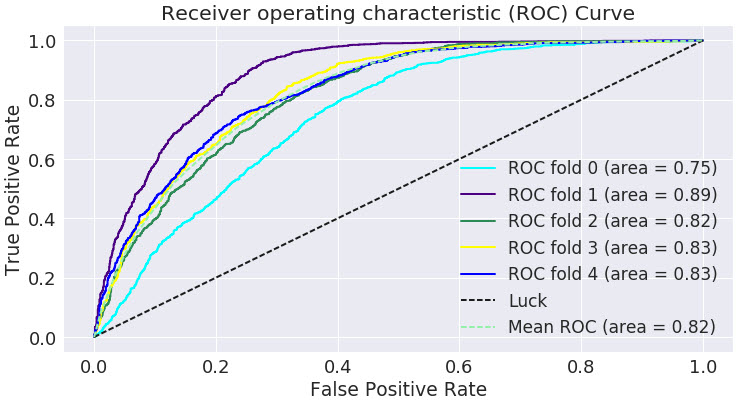
\includegraphics[width=\linewidth]{ROCPlot.jpg}
\caption{Logistic Regression Model Train ROC Curve across 5 folds}
\label{fig:ROCPlot}
\end{figure}

\subsection{Feature Importance Analysis}

\paragraph{While we have briefly discussed the methods used to identify the most impactful variables to be included in our Logistic Regression model, we now discuss these variables and their real-world significance for Human Resource organizations. Only by understanding these features' influence on attrition may organizations hope to curb the rate of voluntary employee separation.}

\subparagraph{Firstly, final features included in our model were, 1) General Schedule Grade, or equivalent (GSEGRD); 2) Lower Limit Age; 3) Bureau of Labor Statistics - 'Other' Industry Separation Rates and number of Job Openings at the time of OPM employee separation; 4) Length of Service (Square Root transformed - LOSSqrt); 5) Various age level bins (Was or was not the employee of an age between 20-24, 40-44, 45-49, 50-54, or 55-59?); 6) Various location indicators (Was or was not the employee residing in Arizona, California, Kansas, Missouri, Montana, New Mexico, Ohio, Pennsylvania, South Dakota, Texas, Virginia, or Washington); 7) Types of Appointment (Was or was not the employee a member of Non-Permanent Competitive Service, Permanent Excepted Service - Schedule A, Permanent Excepted Service - Schedule D, Permanent Excepted Service - Other, Non-Permanent Excepted Service - Schedule B, or Non-Permanent Excepted Service - Schedule C); and 8) Was or was not the employee a member of the Standard Schedule Grade, or equivalent, pay plan (PPGROUP\_11)? These features, and their associated model coefficients, are portrayed in Figure~\ref{fig:Coeffs}.}

\subparagraph{}
\begin{figure}[H]
\centering
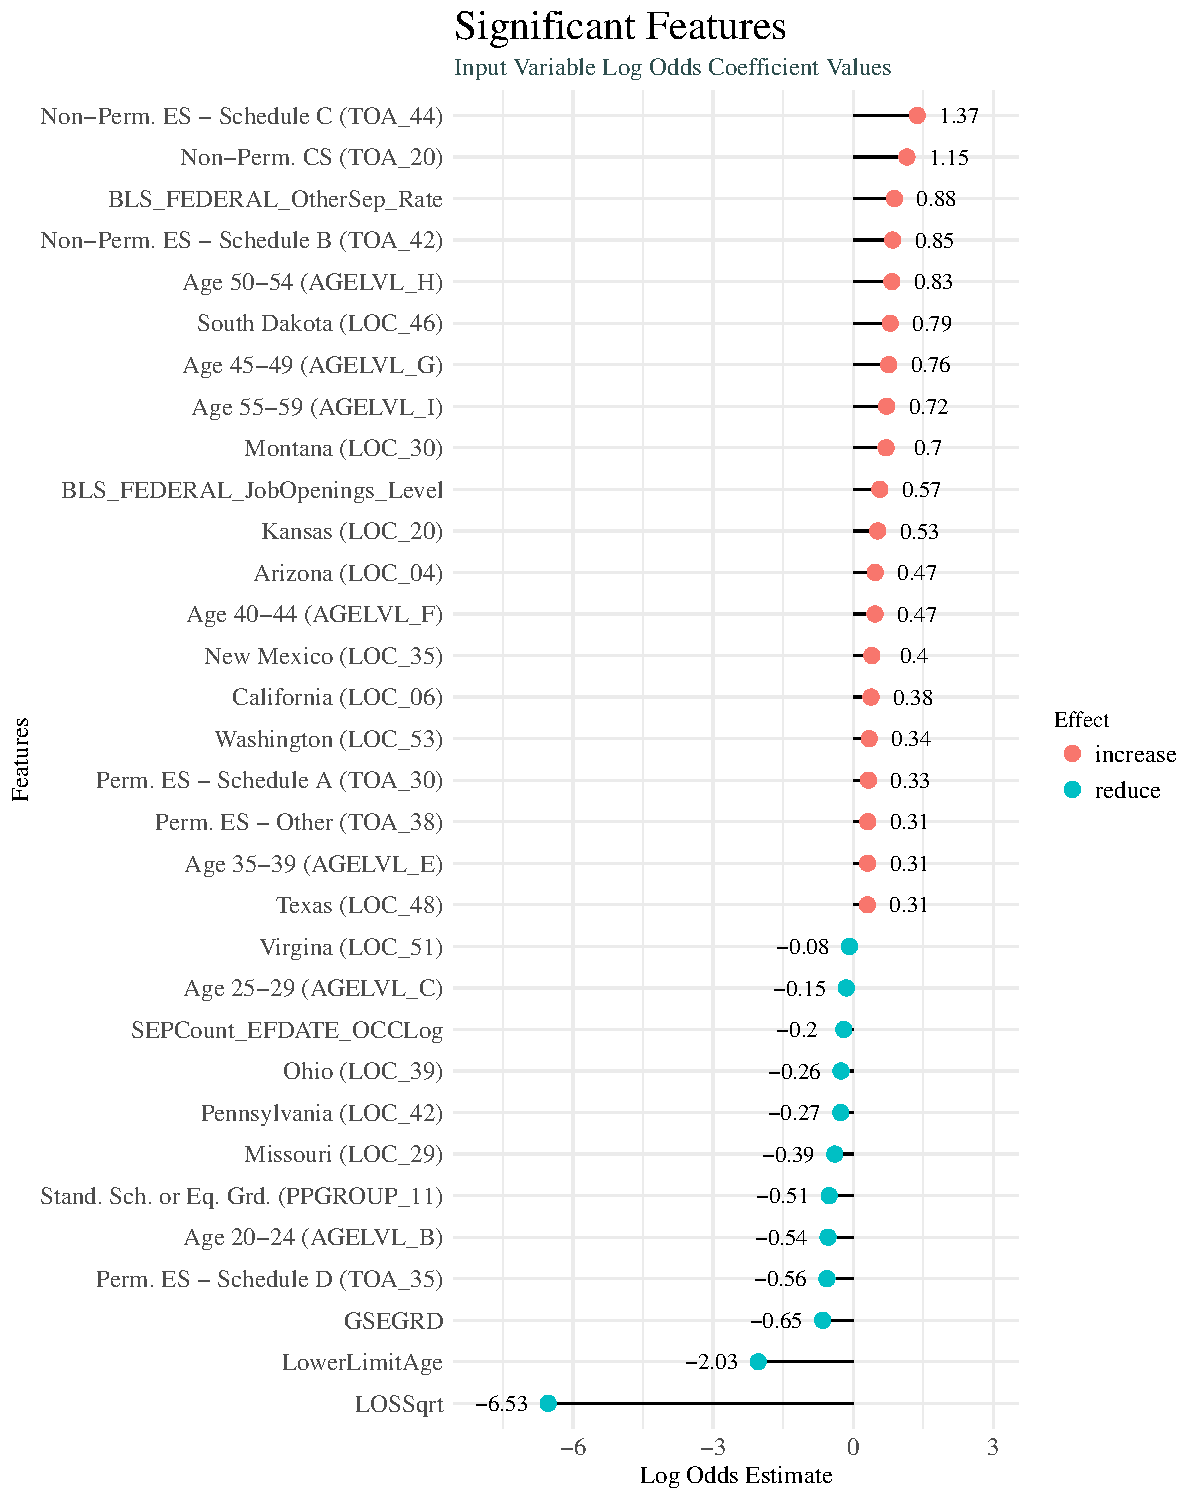
\includegraphics[width=\linewidth]{Coeffs.pdf}
\caption{Statistically Significant Features and Their Log Odds Coefficients}
\label{fig:Coeffs}
\end{figure}

\subparagraph{Given that all variables chosen for final model implementation were statistically significant (p-value $<$ 0.05), coefficients serve as an appropriate means for ranking importance. While all variables were assessed, we choose to focus our current discussion on those attributes we identify as being the most applicable within most every organization, whether in public or private sectors. As such, we first turn our attention to LOSSqrt, the most impactful variable associated with an employee's separation.}

\subparagraph{Each logistic regression coefficient of Figure~\ref{fig:Coeffs} is representative of the change in log odds of the outcome with each one-unit increase for the respective predictor variable. In other words, for LOSSqrt, it is expected that for every one-unit increase in LOSSqrt, the log odds of an employee separating decrease by 6.52 when holding all other exploratory variables constant. As a result, exponentiating this value produces the decrease of odds with each unit increase in LOSSqrt, as indicated in Equation \ref{eq:exp}.}

\begin{equation}
\dfrac{p}{1-p} = e^{-6.52} = 0.00147
\label{eq:exp}
\end{equation}

\subparagraph{This means that with each unit increase in LOSSqrt while holding all other explanatory variables constant, we can expect a 67,757.84\% decrease in the odds ratio (OR) of an employee voluntarily separating! This calculation is portrayed in Equation \ref{eq:delta}.}

\begin{equation}
\Delta OR = \Big(\dfrac{1}{0.001474} - 1\Big)\times100 = 67,757.8385
\label{eq:delta}
\end{equation}

\subparagraph{Since LOSSqrt is a square-root transformation of our original LOS variable, we conclude this change in odds is not linear. For example, a one unit change from LOSSqrt of 1 to LOSSqrt of 2 is equivalent to 3 years' more service ($2^2-1^2=3$), but a change from LOSSqrt of 2 to LOSSqrt of 3 is equivalent to 5 years' more service ($3^2-2^2=5$). So, not only is it clear that the longer an employee stays within his or her company, the far less likely he or she will quit, but also that the strength of years of service diminishes as employees remain employed longer.}

\subparagraph{We next shift our focus to age variables. Intuitively, one might believe these to have a collinear relationship with LOSSqrt; however, as indicated in Figure~\ref{fig:ViolinAge}, such is not the case. Figure~\ref{fig:ViolinAge} facilitates a three-way comparison between the top five most impactful age brackets, separation type, and LOSSqrt; note that brackets are positioned in order of absolute coefficient value with coefficient polarity indicated in parenthesis, violin widths are scaled by count for each 'Yes' or 'No' status, and the three lines in each violin half represent each separation type's Inner-Quartile Range (IQR). While a test for distribution likeness (i.e. t-test) was not performed for each bracket's binary value distributions, visual inspection reveals enough overlap in LOSSqrt values between age bracket binary statuses to suggest independence for older brackets. Understandably, age bracket 20-24 portrays the least amount of overlap since employees of new college graduate age will naturally have fewer years of service.}

\subparagraph{}
\begin{figure}[H]
\centering
\subfloat[First (+ve)]{
  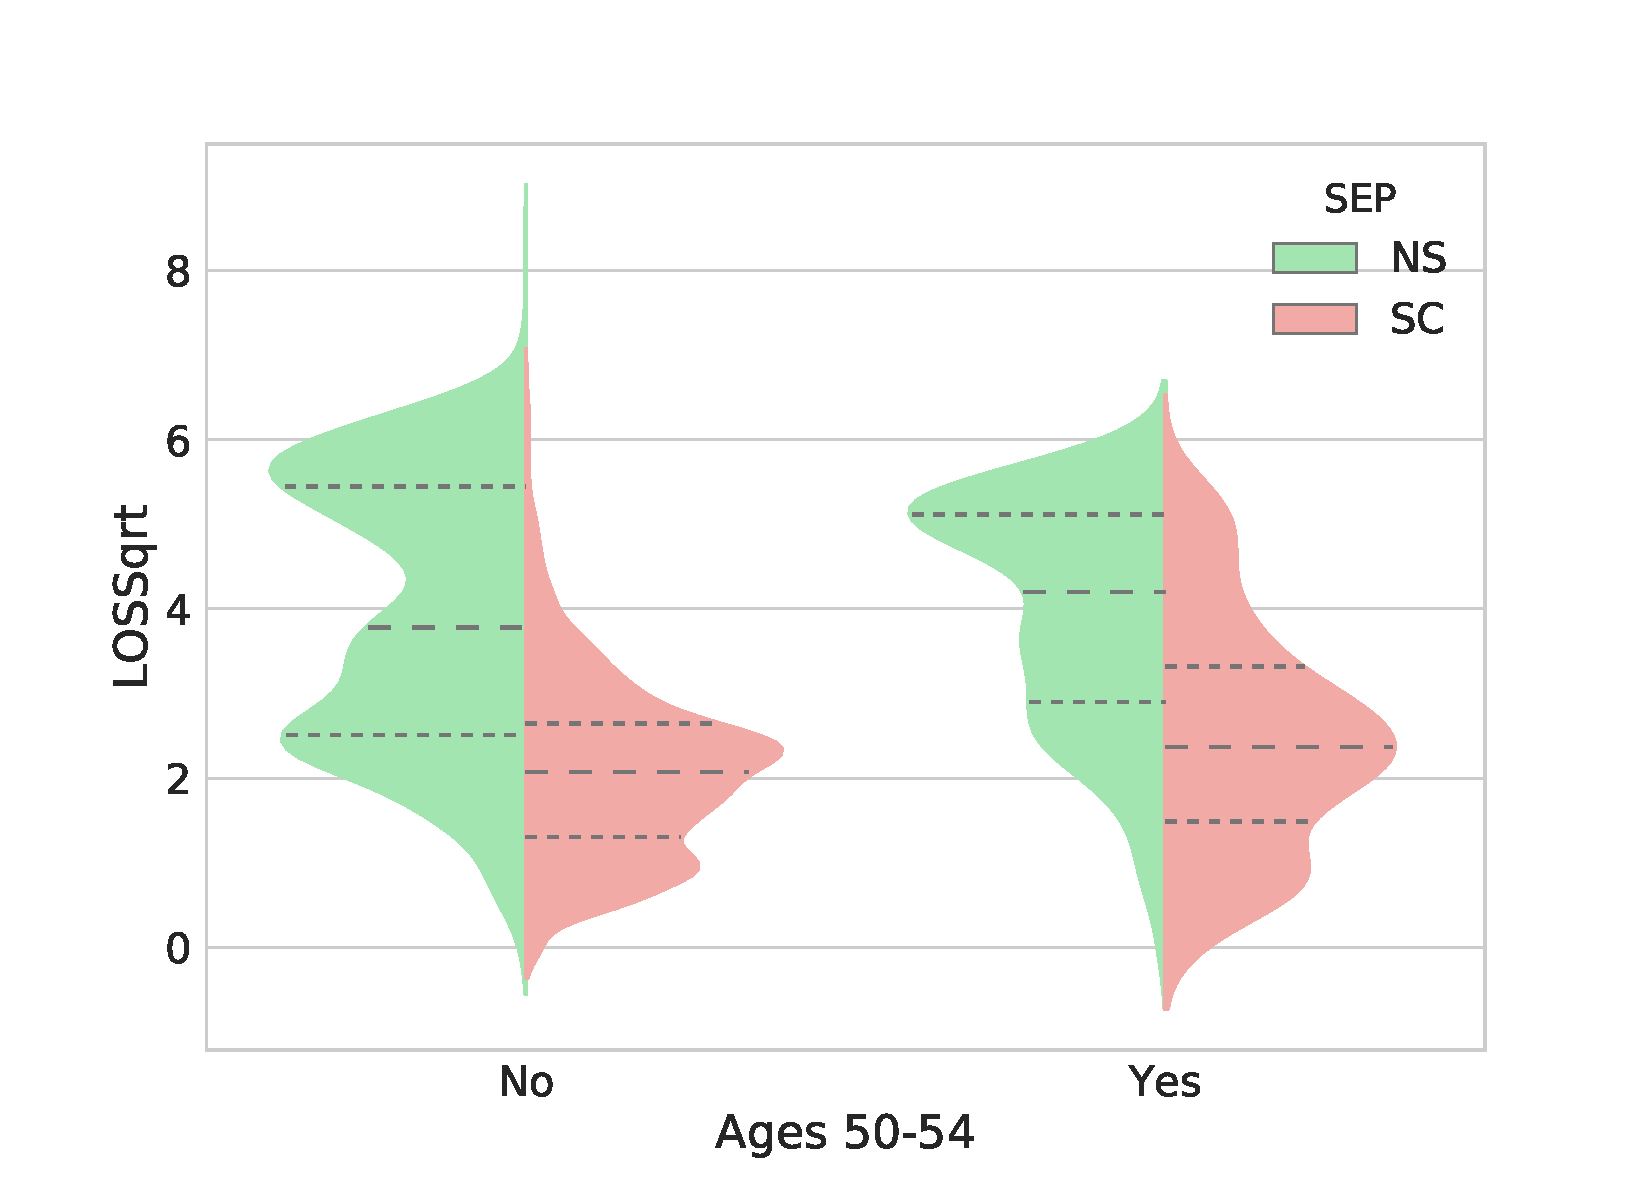
\includegraphics[width=60mm]{Violin_AGELVL_H.pdf}
}
\subfloat[Second (+ve)]{
  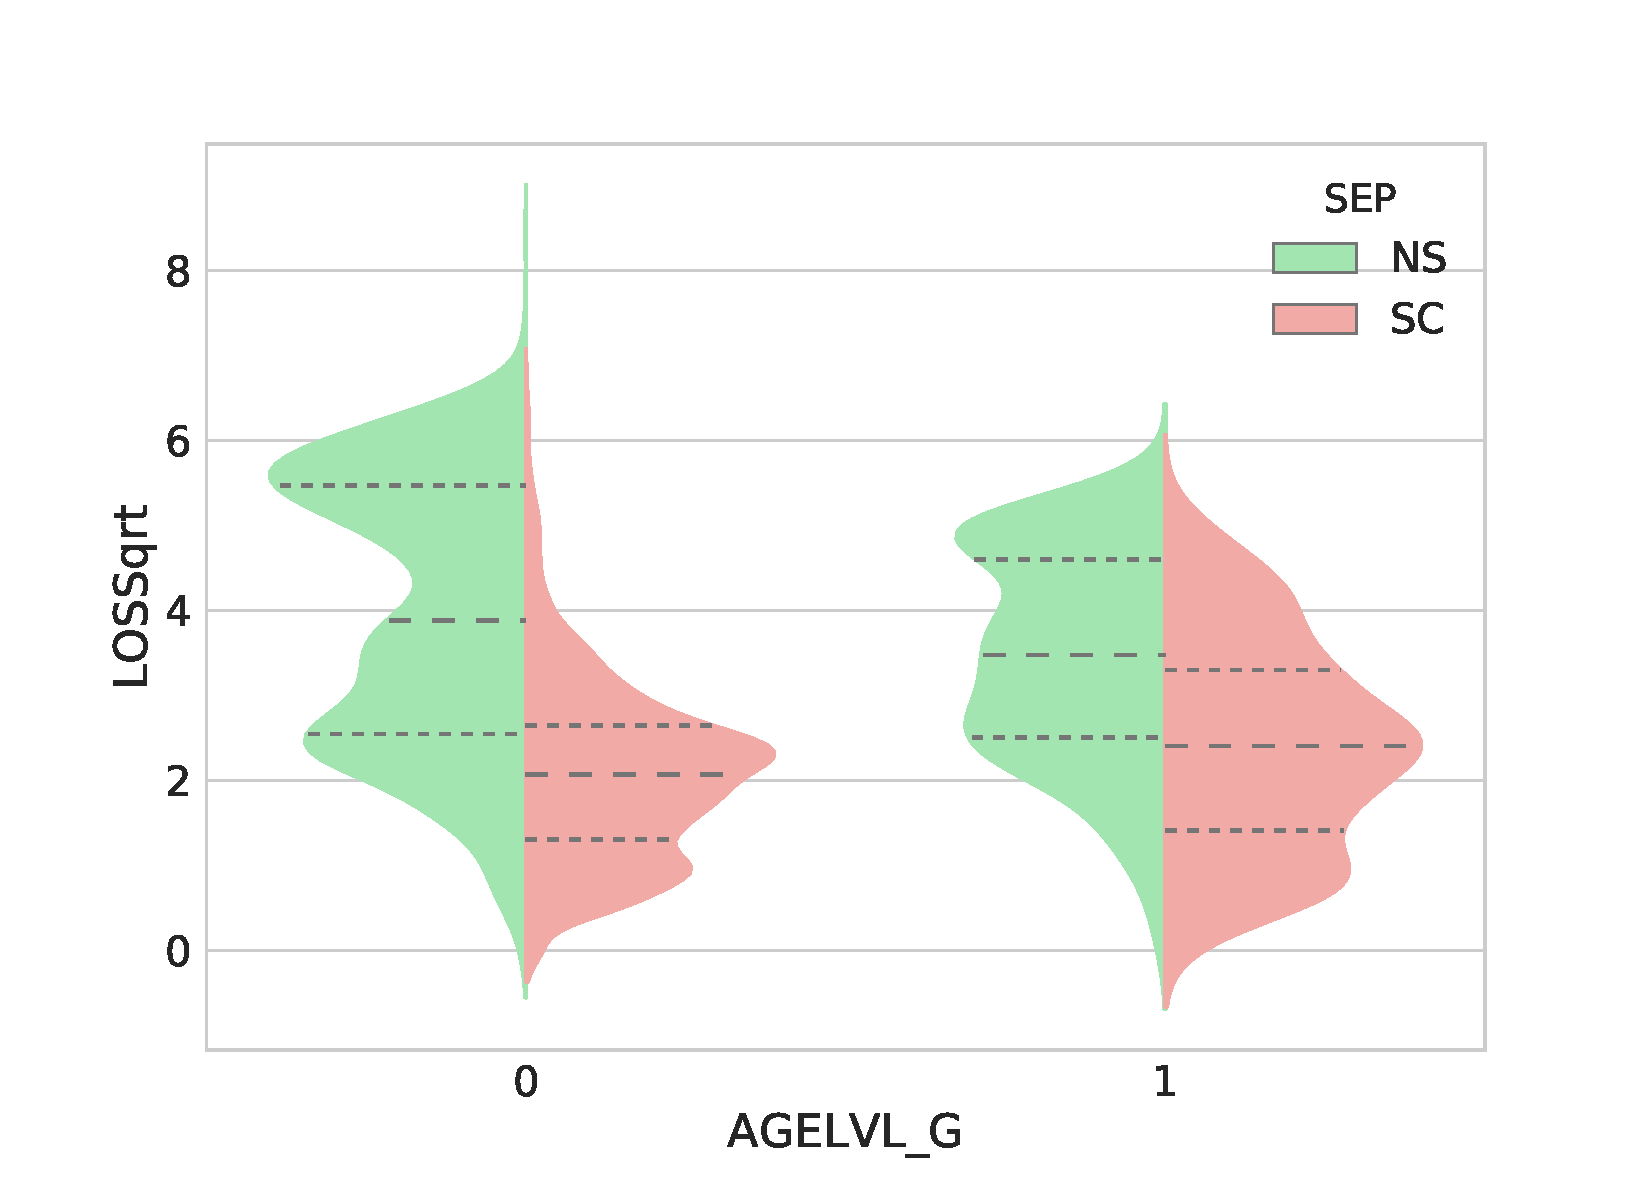
\includegraphics[width=60mm]{Violin_AGELVL_G.pdf}
}
\hspace{0mm}
\subfloat[Third (+ve)]{
  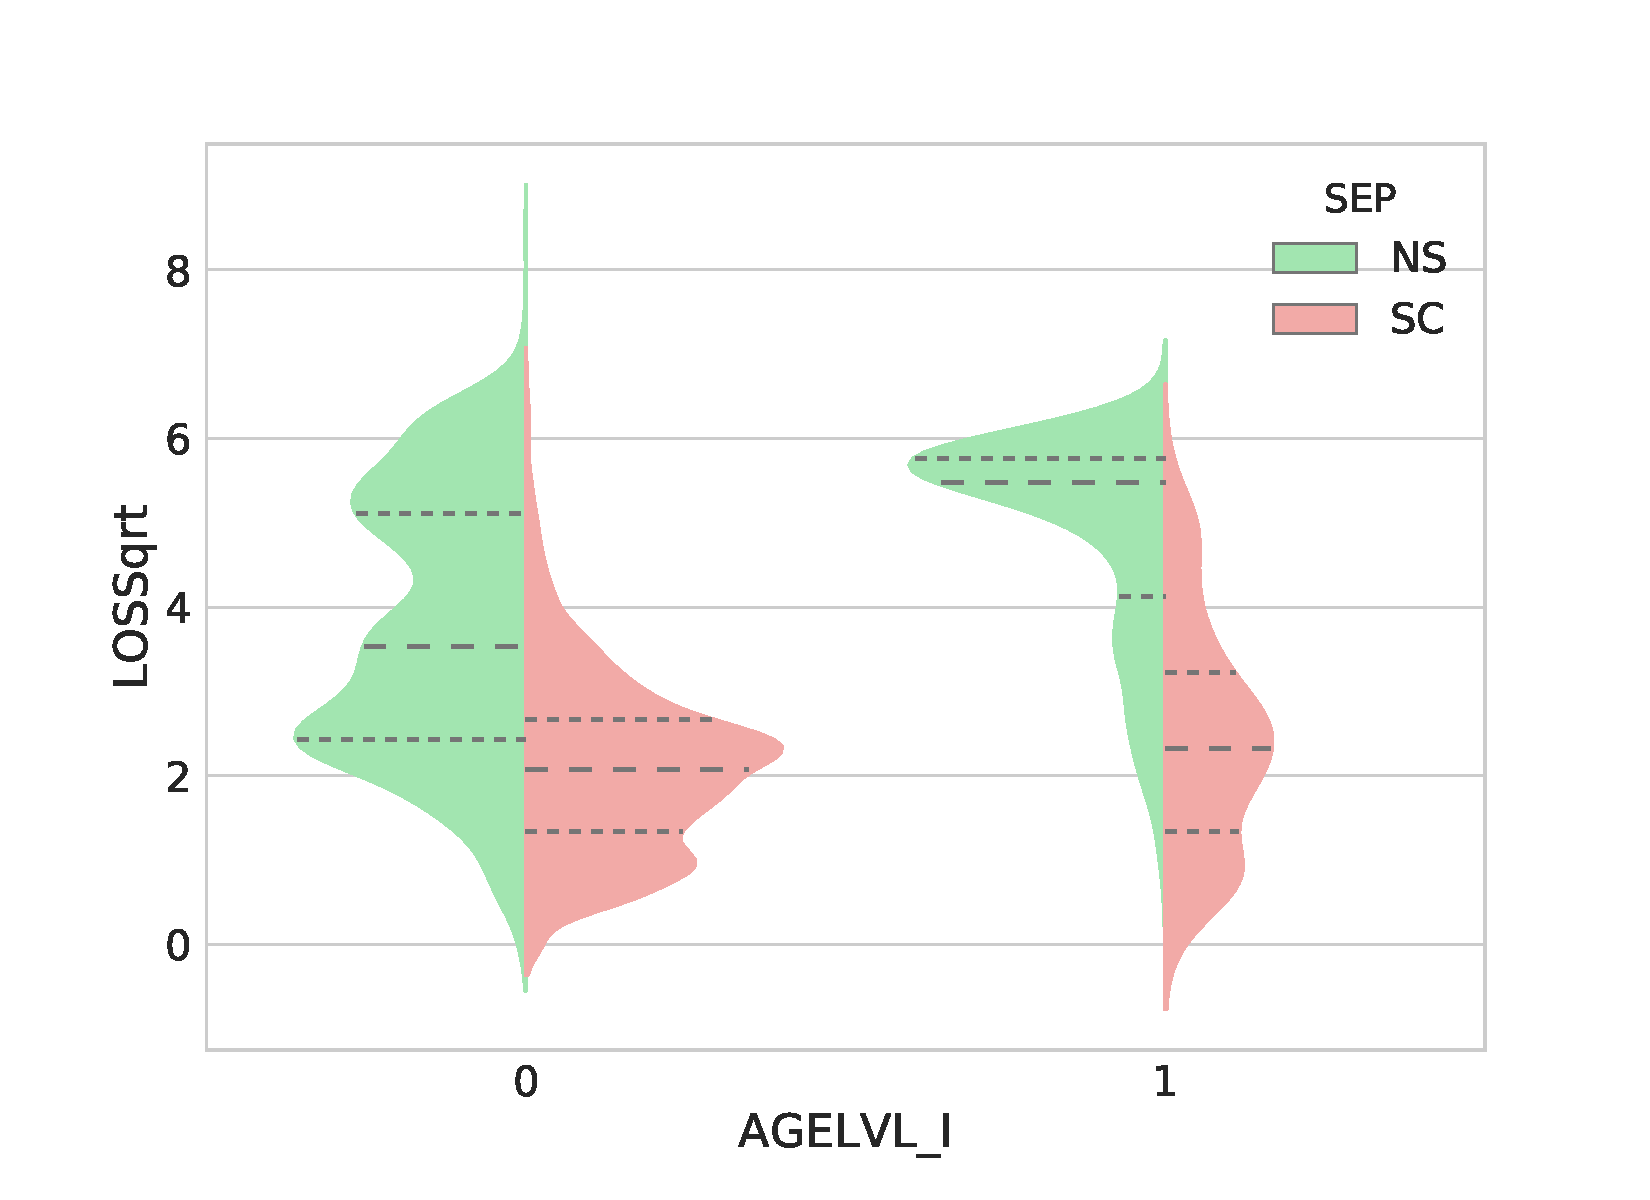
\includegraphics[width=60mm]{Violin_AGELVL_I.pdf}
}
\subfloat[Fourth (-ve)]{
  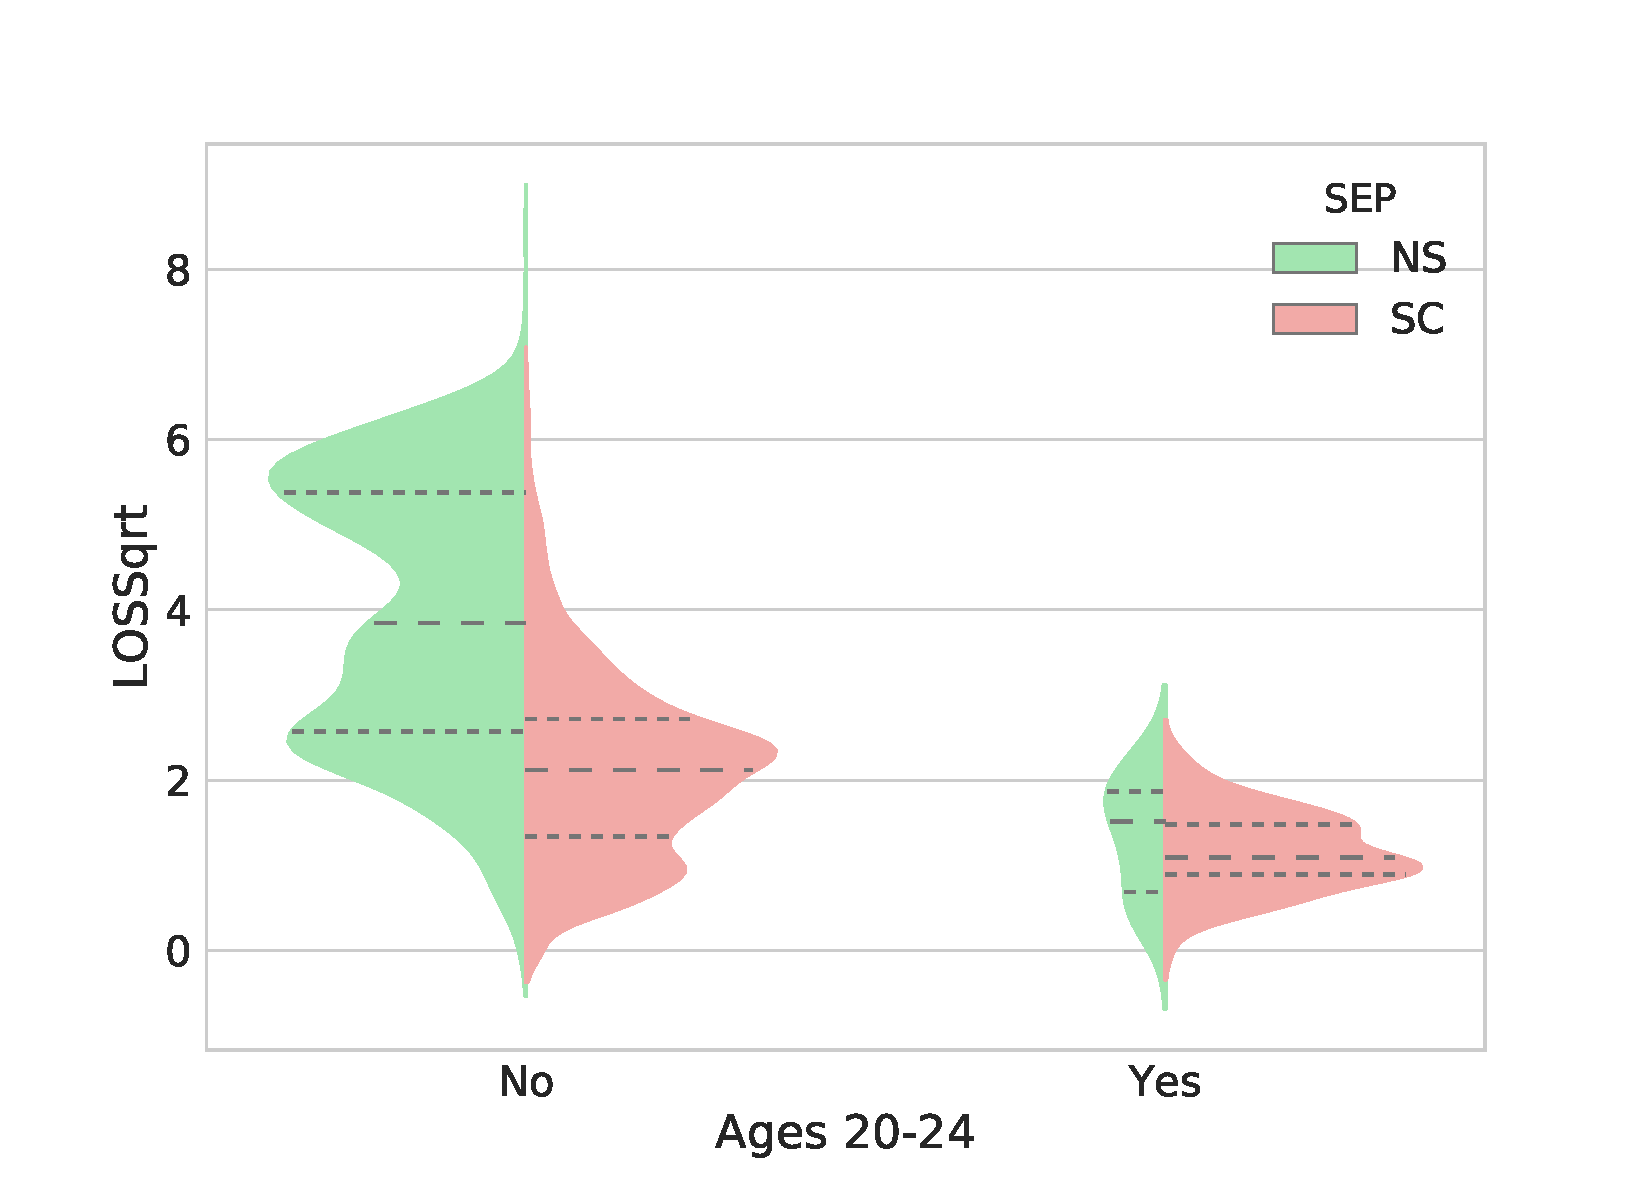
\includegraphics[width=60mm]{Violin_AGELVL_B.pdf}
}
\hspace{0mm}
\subfloat[Fifth (+ve)]{
  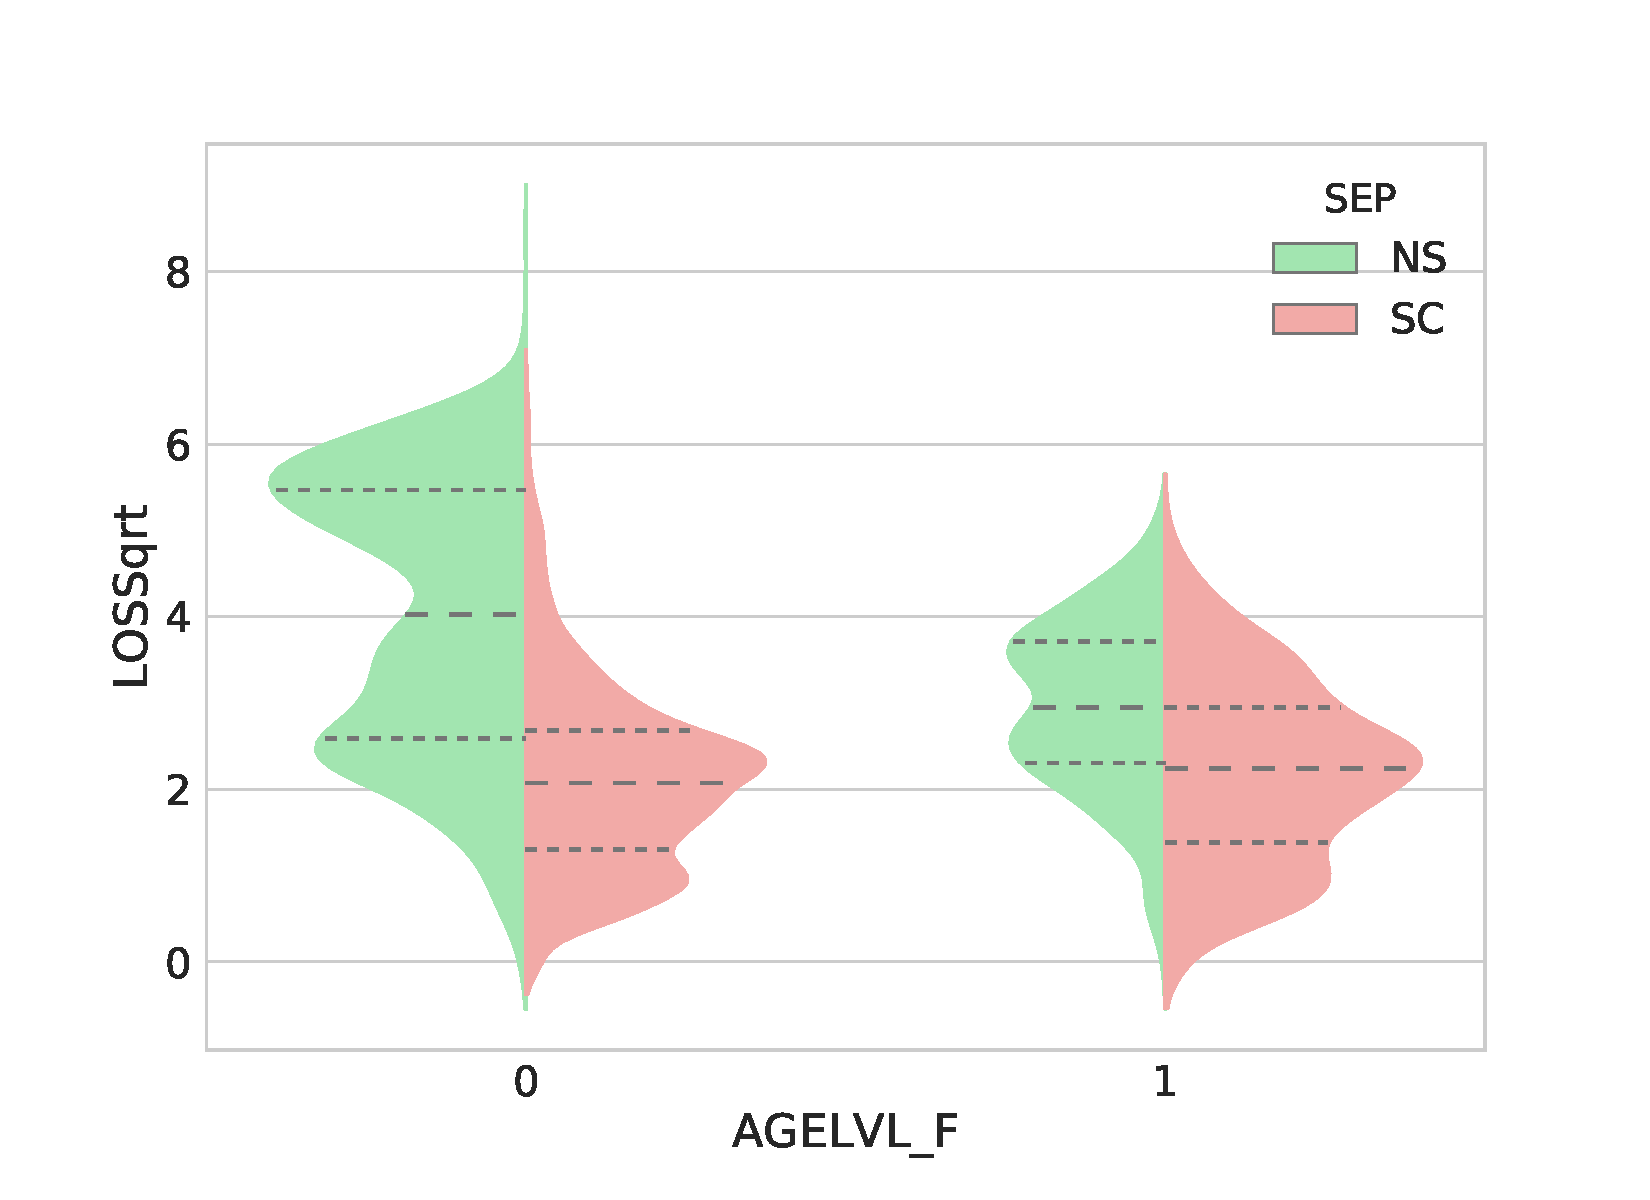
\includegraphics[width=60mm]{Violin_AGELVL_F.pdf}
}
\caption{Violin Plots - Age Levels Ranked by Coefficient Magnitude}
\label{fig:ViolinAge}
\end{figure}

\subparagraph{Figure~\ref{fig:ViolinAge} also reveals that, regardless of age bracket, employees with fewer years of service are more likely to quit. Within these top five age brackets, the 75th percentile of quitting employees (SC) is less than or equal to the 50th percentile among non-separating employees (NS). The most extreme differential is observed among employees belonging to the Age 55-59 bracket, since more than 75\% of those employees who quit have fewer years of service than even 25\% of those who retain their positions.}

\subparagraph{The final assessment among ages when reviewing both Figure~\ref{fig:Coeffs} and Figure~\ref{fig:ViolinAge} is that, when holding all other variables constant, the odds of employees between ages 20-29 voluntarily quitting are actually less compared to older ages, and the odds for employees comprising ages 35-59 are actually increased vs. younger ages. The ages exemplifying virtually no effect on separation type are 30-34 and ages greater than 59. Such relationships in age may seem strange, but when accounting for the strongest effect (length of service), the effects of age extremes are essentially masked.}

\subparagraph{The jittered scatterplot matrix of Figure~\ref{fig:ScatterMatrix} further illustrates the impact of age via the LowerLimitAge variable. The scatterplot and Kernal Density Plot (KDE Plot) comparing LowerLimitAge against LOSSqrt indicate many quits occur at a young age when length of service is minimal and that many non-separations occur at an older age when length of service is high. Most interesting is that quits are not isolated to any particular age, but rather span nearly the entire spectrum of employee ages. Quits do appear to concentrate around 30 years of age and a LOSSqrt value of 2.5 (6.25 years of service), but this has more to do with years of service than it does age based on coefficient values and our previous interpretations (Notice the KDE Plot SC concentration spikes upward in excess of 50 years of age at LOSSqrt = 2.5). It is also worth mentioning the extension of non-separation behavior down into younger ages, concentrating around LOSSqrt = 2.5 as well. Even in the presence of low LOSSqrt, this additional concentration supports Age 20-24 and Age 25-29 model coefficients; the odds of these employees quitting are less than the odds of older employees quitting when holding all other variables constant.}

\subparagraph{}
\begin{figure}[H]
\centering
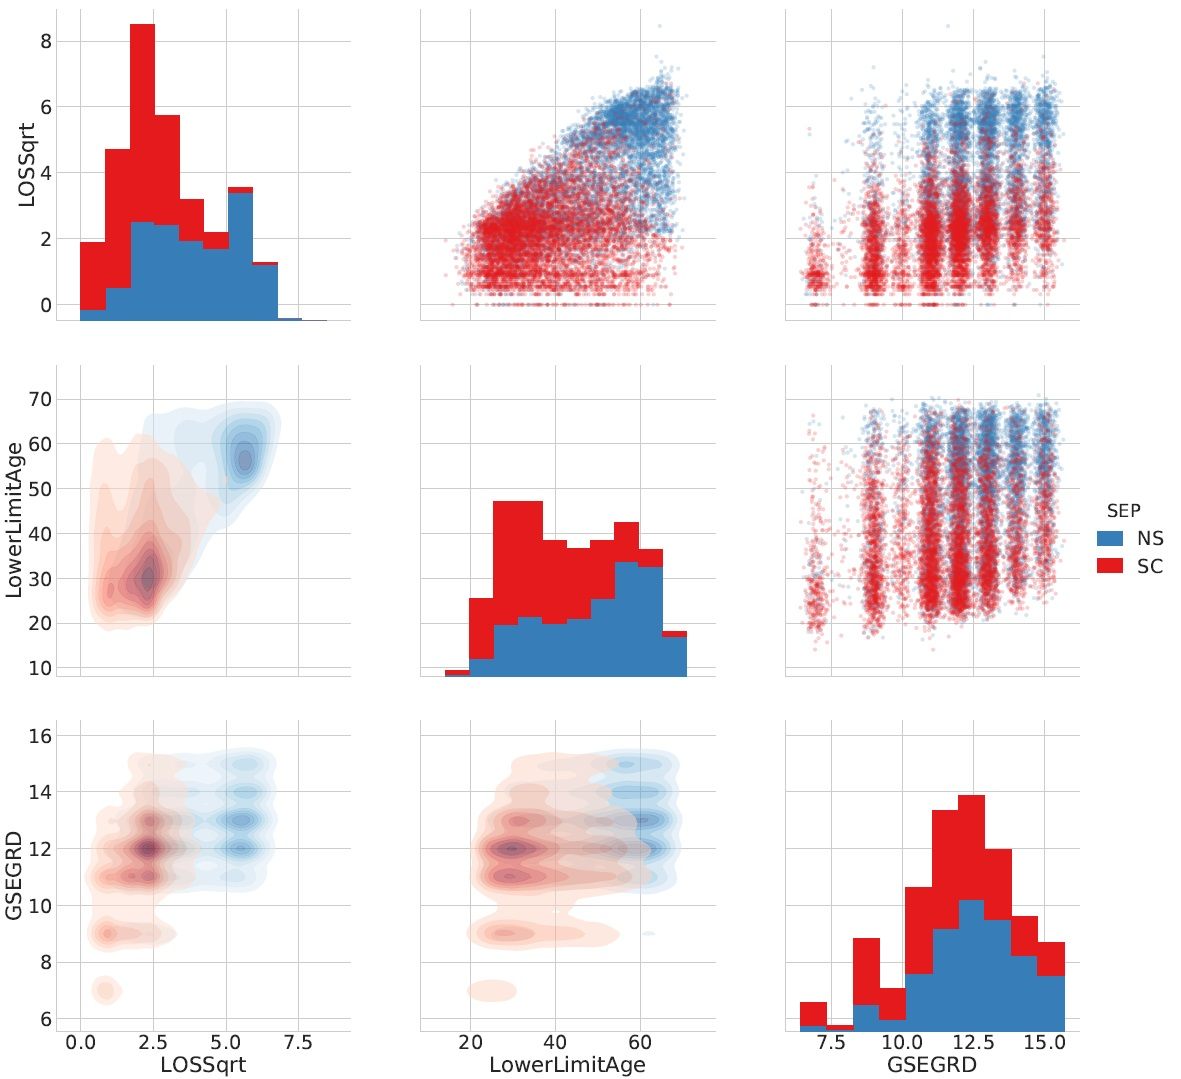
\includegraphics[width=\linewidth]{ScatterMatrix.jpg}
\caption{Jittered Scatter Plot Matrix Results for Top Numeric Attributes}
\label{fig:ScatterMatrix}
\end{figure}

\subparagraph{Figure \ref{fig:ScatterMatrix} also demonstrates the relationship between GSEGRD and LOSSqrt, as well as between GSEGRD and LowerLimitAge. While turnover is expected at lower GSEGRD values, many quits still occur at higher GSEGRD values as well. This supports GSEGRD and LOSSqrt model coefficient relationships as LOSSqrt is far more impactful on employee attrition compared to employee job grade. Comparing GSEGRD and LowerLimitAge supports both GSEGRD and older age bracket coefficients since the frequency of attrition at older ages is more significant when high job grade, and therefore high pay, is less a factor, and attrition is less concentrated among highest paid employees.}

\subparagraph{The last feature we choose to discuss in more detail is PPGROUP\_11: Was the employee a member of the Standard Schedule Grade, or equivalent, pay plan? The log odds estimate for this feature is negative, as indicated in Figure \ref{fig:Coeffs}, so by belonging to this group, an employee is less likely to quit. The violin plots of Figure \ref{fig:ViolinPPGROUP} explore this characteristic further. The Pay Plan Group 11 vs. LOSSqrt plot indicates that while attrition behavior is similar between members and non-members, the mean LOSSqrt value of members who do not separate is nearly 1 unit greater than the mean of non-member NS employees (this amounts to approximately 7 years more service on average when back-transforming LOSSqrt means). This may suggest a joint relationship between LOSSqrt and PPGROUP\_11 and is an area of focus for future model refinement.}

\subparagraph{}
\begin{figure}[H]
\centering
\subfloat[LOSSqrt Distribution]{
  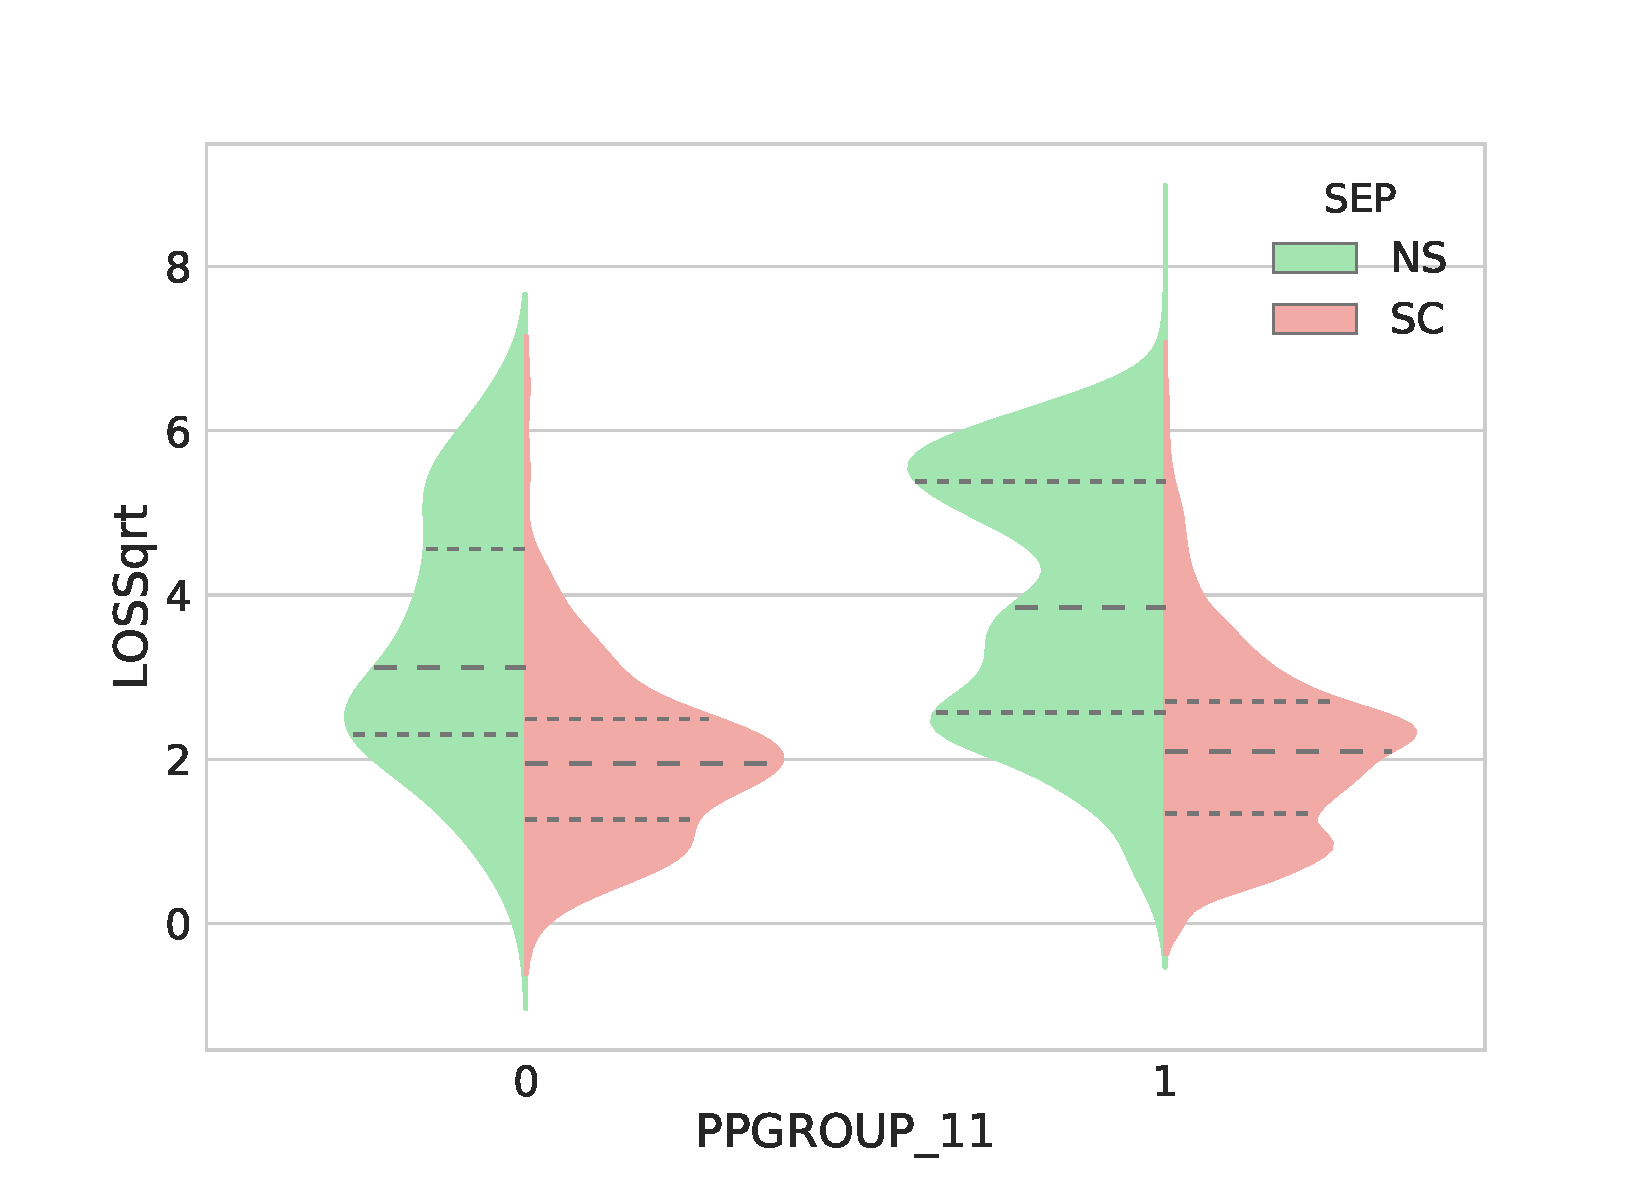
\includegraphics[width=60mm]{Violin_PPGROUP_11.pdf}
}
\subfloat[GSEGRD Distribution]{
  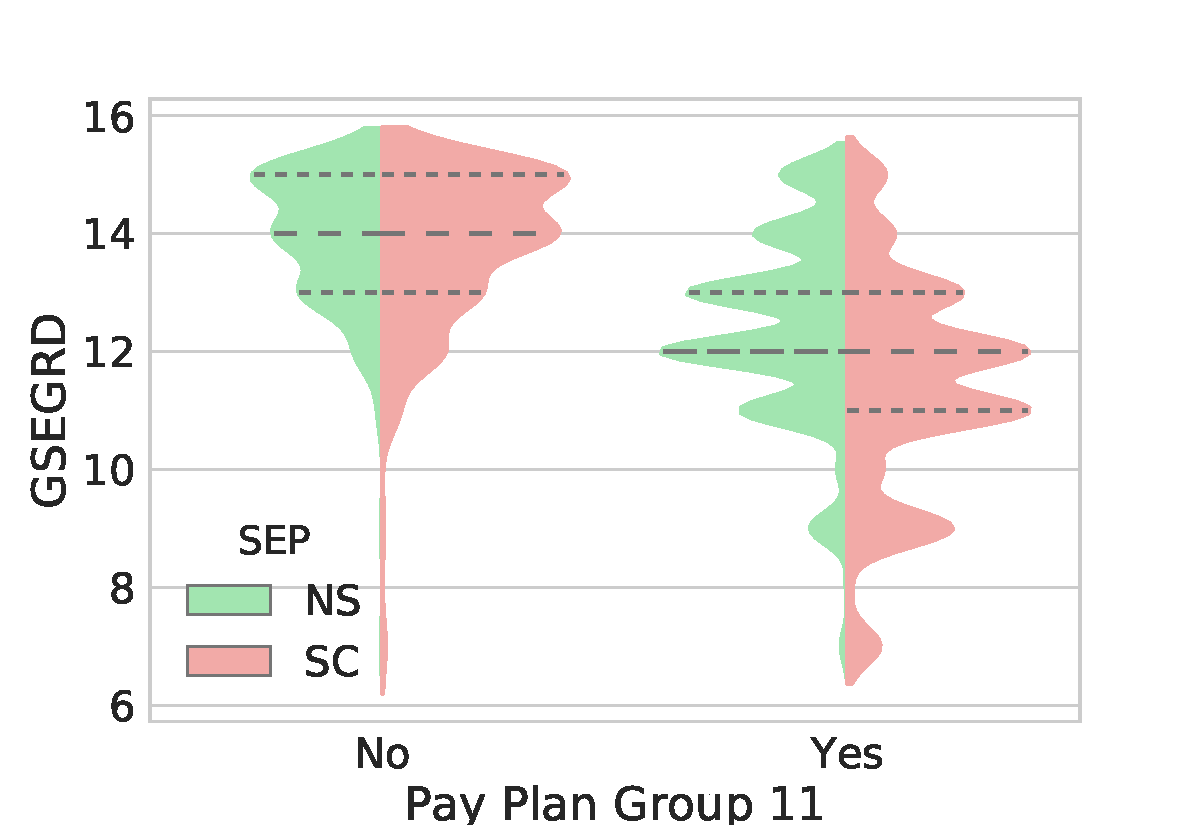
\includegraphics[width=60mm]{Violin_GSEGRD_PPGROUP_11.pdf}
}
\caption{Violin Plot - Pay Plan Group 11}
\label{fig:ViolinPPGROUP}
\end{figure}

\subparagraph{The Pay Plan Group 11 vs. GSEGRD plot of Figure \ref{fig:ViolinPPGROUP} illustrates another differentiatior between group members and non-group members -- pay. Though non-members commonly have higher job grades, it appears they have higher turnover as well. This is interesting given that higher job grades usually represent lower odds for attrition. However, employees not belonging to the standard pay plan are grouped under specialty pay plans such as those for corporate graded employees or physicians and dentists. So, these are specialty employees who may likely have different opportunities available to them outside their public sector industries. More investigation may be required in future works to fully understand such behavior. In the meantime, it suffices us to recognize the disparity between members and non-members of Pay Plan Group 11.}

\subparagraph{While many key features were discussed in this section, type of appointment and location variables were not. This is because while they are important to public sector attrition prediction, they may not be as applicable in private sectors. Due to these differences and the varying counts of employees present in each appointment type and location, we plan to revisit our sampling methodology in the future to improve broader application and accuracy.}


\subsection{Test Scope Expansion to Administrative Occupations}

\paragraph{Training our model once more, utilizing the entire sampled data set instead of selecting merely one of the 80/20 train/test splits, the model fit was saved for consumption on additional data from the Administrative occupation category. This test allows us to assess whether our model holds true across varying occupation families. This model was applied to administrative data, which underwent the same sampling strategy as was performed for professional occupations. Upon reviewing Figure~\ref{fig:AdminLRConfus}, we found results are nearly identical to that of the professional training tests. We may see that of all administrative individuals who quit (SC), we predicted 72\% of them correctly, and only 26\% of Non-Separation (NS) individuals were incorrectly associated as likely to quit. Although we have misrepresented these Non-Separation individuals, there may be relevance to their prediction. If this is a job satisfaction issue, than this might require a shift in leadership to help prevent future turnover. Between both the True Positive and False Positive quit predictions, there could be some value in these insights to an organization. These results could identify a target demographic for further assessment to help understand what action could be taken to help reduce attrition in the workplace. Although this model appears to hold its value across both professional and administrative occupations, one must tread carefully to expand the scope of reach even further. Similar tests and analysis need conducted for expanding this model's reach past these two groups, as findings may be different for other occupation categories.}

\subparagraph{}
\begin{figure}[H]
\centering
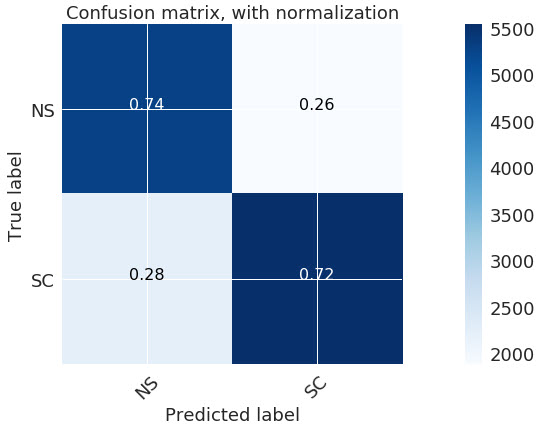
\includegraphics[width=.8\linewidth]{AdminLRConfus.jpg}
\caption{Confusion Matrix Results for Predicting Administrative Occupations Results}
\label{fig:AdminLRConfus}
\end{figure}

\section{External Validation}

\paragraph{Our model is based on features made public through the Federal Office of Personnel Management and the Bureau of Labor Statistics.  As such, we expected to see limitations in the validity of our model for private sector companies. A part of our concern was in the fact that we would not have additional data to which an HR office might have access, such as self-reporting surveys on job satisfaction, work-life balance, and even performance reviews. In an effort to produce as accurate a model as possible, we sought out other sources that might provide insight into how such variables might impact the attrition rate.}

\subparagraph{IBM released a data set in 2015 that contains 35 features with a categorical response variable for Attrition as "Yes" or "No" \cite{stacker}. This data set is "based [off] real data with all personal identifiers removed," but was "also tweaked so that it performs better in telling a story about attrition" \cite{watson}. This data was provided as part of an IBM Watson Analytics promotion to push their new analytics platform. IBM also provided a sample use-case scenario for the data set wherein they identified the primary features correlated to attrition as well as determined the attrition rate for several demographic categories of employees \cite{alexander}.}

\subparagraph{While the data provided by IBM had been "tweaked" \cite{watson}, it was based on anonymized, real-world data, and still provides insight into what data is considered valuable by IBM Watson Analytics in defining and predicting employee attrition. To this end, we performed exploratory data analysis to verify the findings of the IBM Watson Analytics group, as well as compare the strongest features of this data set with the features selected for our model.}

\subparagraph{}
\begin{figure}[H]
\centering
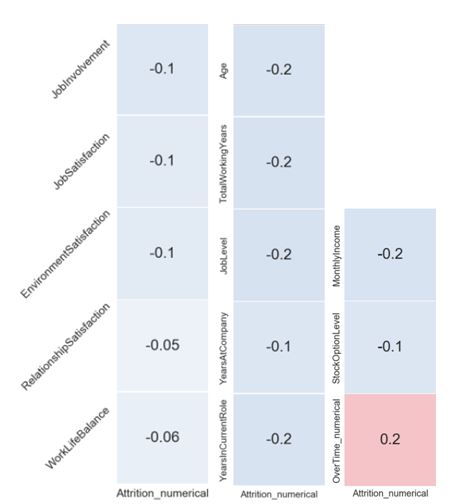
\includegraphics[width=.8\linewidth]{IBMSepCorr.jpg}
\caption{IBM Attribute and Separation Correlation Values}
\label{fig:IBMSepCorr}
\end{figure}


\subparagraph{In Figure \ref{fig:IBMSepCorr} are the results of a simple Pearson's r correlation review for several features against attrition. The features with the highest correlation are those concerning age, duration of employment, and economic factor such as monthly income and whether the employee participated in overtime. Qualitative features, such as environment and job satisfaction, are correlated to attrition, but not to the same degree of the other factors. From what we know in our analysis of the OPM data set, length of service is, by far, one of the most important variables we found in building our model for predicting employee retention, and we see a similar negative correlation here in the IBM data set. After length of service are variables pertaining to age, and pay grades. This further parallels what we see within the IBM data set - the direction of correlation, if not necessarily the magnitude.}

\subparagraph{With the IBM data set comparison, we are on the right track for our model, but there is a glaring weakness that the IBM data set reveals in regards to the publicly available OPM data set. That is in the qualitative factors. Modeling the relationship between length of service, pay scale and age gets us most of the way, but there is nuance to the difference between individuals at equivalent levels for each feature.  These differences are probably to be found in measuring satisfaction, work life balance and even engagement. For millennials, 60\% are open to different job opportunities, but 26\% are less likely to leave if they are engaged at their current place of employment \cite{gallup}. This seems to reflect the fact that, for disengaged employees, 54\% would leave their current position for a pay increase of 20\% or less, whereas only 37\% of engaged employees would do the same \cite{gallup2}.}

\subparagraph{Based on our findings with the OPM data set, we have identified key features of employees considering leaving their position and built a model with reasonable accuracy for identifying those individuals. These features have corroboration with sample data sets made available online, but we do recognize that our model could be further improved by the addition of qualitative components to better predict attrition rates since there is room for variance between two individuals in similar economic and duration circumstances.}
 
\section{Ethical Considerations}

\paragraph{At the crux of any activity that collects and interprets data on human behavior is the question, "Who is to benefit, the gatherer or the subject?" Would our model prompt a company to strive for increased employee tenure, or would it reduce compensation and other benefits once it is aware of an employee’s "shelf life?" We touch upon several of these ethical dilemmas below.}
 
\subsection{Size of the Interested Party}

\paragraph{One of the benefits of using third party data is that a smaller organization does not risk breaking anonymity. For example, maintaining anonymity in a smaller size company (e.g. one or two employees per department) would be outside the realm of possibility should the organization gather such data as presented herein. However, by using data from such a large entity as the US Government, a Human Resources professional would be able to gain insight about the departments in their company without risking important employee relationships.}
 
\subparagraph{That being said, the data we analyzed is applicable to employee groups as a whole, not individually. There are many factors that could impact an employee choosing to leave, and when big data is applied to small departments or single individuals, an HR professional might incorrectly assume that one of their employees will act similarly to the behaviors of general groups. In reality, an employee’s family life, manager, financial situation, and perception of self-worth may drastically affect the outcome of applying large-scale behavioral models to small populations.}
 
\subsection{Reliability and Unintended Consequences}

\paragraph{In the case where employee disclosure is required as part of the data gathering process (e.g. the performance data from the IBM data set), an employee may not feel comfortable being completely honest about certain attributes. For example, if an employee is to rate their job satisfaction, would said person be concerned that their results would be seen by a manager and used against them? Would the realization that he or she is not satisfied prompt them to then begin a job search? The reliability of such qualitative data is certainly subject to scrutiny.}
 
\subparagraph{Additionally, any data that is to be collected would need to be stored and used in an ethical and safe manner.  Risks such as lack of anonymity, improper use, and reactions from employees whose data is being collected are only a few of the concerns to be addressed. Certainly, the collection of employee data such as length of service, years to retirement, etc., are features that are not very attributable to individual respondents. For these reasons, if a company wishes to gain insight into the attrition rate of their own employees, it would be advisable to either, 1) form an internal team or committee to monitor and advise on the collection of employee data, and 2) perhaps bring in a third-party researcher that will commit to maintaining anonymity and autonomy.}
 
\subsection{Improving the Life of an Employee}

\paragraph{Making inferences of what prompts an employee to leave should be checked against whether the lives of the employees are actually improved. A company that is wanting to simply reduce attrition cost might actually commit unethical acts if they do not take a comprehensive approach to this practice.}

\subparagraph{For example, if gender is collected as part of a survey, perhaps an employee attrition model finds that women have a higher attrition rate than their male peers. If we build our model around that feature, we then are at risk of making the statement that gender is just as important as, say, salary when determining attrition rate. Even though gender may have societal associations that would result in attrition, it would be considered morally reprehensible if those associations were taken into consideration for hiring practices.}
 
\subparagraph{Also, consider the ever elusive "work/home life balance." If personal events are found to affect employee attrition, then the question becomes, "Is that something for which a Human Resources or Management professional should be screening candidates?" There is a possibility that such data can impact the model, and while there is likely quite a bit of improvement that may come from collecting such data, the risk of the bias that could come of it is ever present.}
 
\subsection{Systematic Propagation of Unfair Practices}

\paragraph{A glaring ethical challenge from employing an attrition model is the chance that, once trends are realized, a company actually instills processes that create systematic disadvantages for its employees. For example, say a company learns that individuals aged 30-45 years, working in marketing departments, average three years at their employer and are often underpaid in relation to their industry when they quit. In response, the company updates its profit sharing plan to only vest for its employees once they have reached five years of service. Rather than keep more employees around, the company inadvertently created more discontent, profiting by keeping unvested profit sharing contributions and continuing to pay their workers less than the industry average.}

\section{Conclusion and Additional Research}

\paragraph{With correlations in mind, we performed modeling using Random Forest, K-Nearest Neighbor, and Logistic Regression.  The ninety-nine features were reduced to simplify the model and narrow the interpretation to the largest contributing variables.  In reviewing the model’s most impactful features, we uncovered 1) a significant reduction in odds of an employee quitting as his or her service length increases, 2) odds increase or decrease depending on employee age, and 3) odds of quitting are less if the employee is in the standard pay plan. Comparing age and length of service, we found quits spike around 6.25 years of service, regardless of age. Ultimately, it was logistic regression that gave the highest accuracy, predicting employee attrition with over 74\% success.}

\subparagraph{Of course, as one might expect, predicting employee attrition is not straightforward.  Multiple factors affect each other in different ways and at different levels of existence.  The challenge of finding enough reliable data to analyze was answered with the OPM, BLS, and IBM data sets, enabling us to sample effectively and employ multiple modeling techniques.  The process was iterative, going back to previous steps to respond to certain results (or lack thereof).  Ultimately, the produced model incorporates a rigorously developed and tested set of variables.}

\subparagraph{There are additional areas to research and investigate from here.  One might want to take this model, and determine the impact of location (LOC) and whether or not it can be altered or removed.  Many organizations will not have employees in every state, and therefore, location would need to be analyzed further.  This is not to say that the answer is to simply remove location as a variable if an organization simply does not have employees in all fifty states.  The ability to transfer to other states and keep the same position would imply the location variable should be removed, but particularly competitive geographic areas would indicate that there is a location effect that should remain included. One alternative to location as a categorical variable would be to incorporate income inflation percentages into our analysis, as several state schedule grades have a locality margin applied to accommodate for variations in local expenditures. These locality salary inflation margins may account for some of the confounding variables at play, not accounted for in our current model. Additionally, the effects on age, although impactful to the model, may benefit from true age values versus the provided age bins as were utilized in this analysis. Using raw values may provide a lower margin of error and potentially increase the value of insights provided versus the utilization of bins and "Lower Limit Age".}

\subparagraph{Another area of further research would be to explore other employment data. One such application would be to explore employee perceptions of various employment benefits.  For example, the future retirement benefit certainly played a role in the data used for this paper.  The impact of differentials in income, if present, could have been negated by an employee's knowledge of a future benefit.  Collecting data on employee attrition where the employee had no pension set aside, or perhaps a general survey of employee perception of various retirement benefits, would help to further understand the effect of future pension income on a decision to quit.}

\subparagraph{Finally, applying this model should certainly be used with an ethical lens. If its use does not provide value to employees’  lives, then this would indicate that employee retention is only in the interest of the employer. Responses to any model findings should include considerations on who stands to benefit from such model implementation, and which responses to these findings will actually improve the lives of employees. Otherwise, an organization stands to retain sensitive data that could cause more harm than good. If used diligently, this model offers to help an organization improve profitability, while aligning its goals with those individuals who work for them.}  

\subsubsection*{Acknowledgements}

\paragraph{The authors would like to thank FedScope for their support in helping to understand the OPM data, and Sherry Vitovsky, formerly of AAFES, for her contributions to this project.}

 
\nocite{*}
\printbibliography


\end{document}